\documentclass[12pt,letterpaper,reqno]{amsart}
\usepackage{enumerate}
\usepackage[shortlabels]{enumitem}
\usepackage{graphicx}
\usepackage{amssymb}
\usepackage[normalem]{ulem}
\usepackage{titlesec,bbm, hyperref}
\usepackage{spverbatim} 
\usepackage{esvect}
\usepackage{geometry}
\usepackage{caption}
\usepackage{subcaption}
\usepackage{tkz-euclide}
\usepackage{pgfplots}
\usetikzlibrary{arrows.meta}
\geometry{letterpaper, portrait, margin=0.5in}

\newcommand{\N}{\mathbb N}
\newcommand{\Q}{\mathbb Q}
\newcommand{\Z}{\mathbb Z}
\newcommand{\id}{\mathrm{id}}
\pgfplotsset{compat=1.15}
\begin{document}

\thispagestyle{empty}
\begin{center}\large{
    MATH 621\quad
    HW 1\quad
    Sumanth Ravipati\quad
    February 4, 2019}
\end{center}
\vspace{.15in}
\begin{flushleft}
Note: No sources or people used to complete this assignment
\end{flushleft}
\vspace{.25in}

\begin{enumerate}
\item[1.] Let $f : A \rightarrow B$ and $g : B \rightarrow C$ be functions. Prove the following implications:\newline
\begin{enumerate}
\item If $f$ and $g$ are injective, then $g \circ f$ is injective.\newline
\begin{flushleft}
We wish to show that $(g \circ f)(a) = (g \circ f)(b) \Rightarrow a = b$, which implies that $g \circ f$ is injective. If $(g \circ f)(a) = (g \circ f)(b)$, it is equivalent to $g(f(a)) = g(f(b))$. Since $g$ is injective, $g(f(a)) = g(f(b)) \Rightarrow f(a) = f(b)$. Since $f$ is injective, $f(a) = f(b) \Rightarrow a = b$. Therefore, $(g \circ f)(a) = (g \circ f)(b) \Rightarrow a = b$, as desired. $\Box$
\newline
\end{flushleft}
\item If $f$ and $g$ are surjective, then $g \circ f$ is surjective.\newline
\begin{flushleft}
We wish to show that $\forall c \in C, \exists\, a \in A$ s.t. $(g \circ f)(a) = c$, which implies that $g \circ f$ is surjective since $g \circ f: A \rightarrow C$. Since g is surjective, for a given $c \in C$, we know that $\exists\, b \in B$ s.t. $g(b) = c$. For a given $b \in B$, we know that $\exists\, a \in A$ s.t. $f(a) = b$. Since $g(b) = c$ and $f(a) = b$, $g(f(a)) = g(b) = c$. Therefore, for a given $c \in C$, $g(f(a)) = c = (g \circ f)(a)$ or equivalently, $g \circ f$ is surjective. $\Box$
\newline
\end{flushleft}
\item If $g \circ f$ is injective, then $f$ is injective.\newline
\begin{flushleft}
We wish to show that $f(a) = f(b) \Rightarrow a = b$. Let $f(a) = f(b)$ and evaluating both using the function $g$ gives us $g(f(a)) = g(f(b))$. Since $g \circ f$ is injective, this implies that $a = b$ . Therefore, given $f(a) = f(b)$, we have shown that this implies that $a = b$, which is shows that $f$ is injective. $\Box$
\newline
\end{flushleft}
\item If $g \circ f$ is surjective, then $g$ is surjective.\newline
\begin{flushleft}
We wish to show that $\forall c \in C$, $\exists\, b \in B$ s.t. $g(b) = c$. If we let $c \in C$, we know that $\exists\, a \in A$ s.t. $(g \circ f)(a) = c$, since $g \circ f$ is surjective. Let the function $f$ map that element $a$ to $f(a) = b$, where $b$ is some element in $B$. $(g \circ f)(a) = c \Leftrightarrow g(f(a)) = c$ and since $f(a) = b$, $g(b) = c$, $\exists\, b \in B$ s.t. $g(b) = c$. $c$ was an arbitrary element of $C$ and so we can see that $\forall c \in C$, $\exists\, b \in B$ s.t. $g(b) = c$, and therefore $g$ is surjective. $\Box$
\newline
\end{flushleft}
\end{enumerate}
Then give an example of functions where $g \circ f$ is injective but $g$ is not, and where $g \circ f$ is surjective
but $f$ is not.\newline
\begin{flushleft}
Let $A = \{a_1\}, B = \{b_1, b_2\}, C = \{c_1\}$ and let $f: A \rightarrow B$ and $g: B \rightarrow C$ where $f(a_1) = b_1$ and $g(b_1) = c_1$ and $g(b_2) = c_1$. Since there is only one element in $A$, $g \circ f$ can only map $a_1 \in A$ to $f(a_1) = b_1 \in B$ and then to $g(b_1) = c_1$. Therefore, $(g \circ f)(a) = (g \circ f)(a^\prime) \Rightarrow a = a^\prime$ since $a = a_1 \forall a \in A$. However $g$ is not injective since $g(b_1) = g(b_2) = c_1$, but $b_1 \not= b_2$. $g \circ f$ is surjective since $\exists a_1 \in A$ where $(g \circ f)(a_1) = g(f(a_1)) = g(b_1) = c_1$. This is true for all elements in $C$ since there is only 1 element in $C$. $f$ is not surjective since $\not\exists a \in A$ s.t. $f(a) = b_2$. We can easily verify this by checking the only element in $A$: $f(a_1) = b_1 \not= b_2 \in B$.
\newline
\end{flushleft}
\newpage
\item[2.] For a function $f : A \rightarrow A$ denote by $f^n$ the composition $f \circ \cdots \circ f$ ($n$ times). Show that if for each
$x \in A$ there is an $n(x) \in \N$ such that $f^{n(x)}(x) = x$, then $f$ is bijective.\newline

\begin{flushleft}

We shall show that $f$ is bijective by showing that it has an inverse. We are given that for each $x \in A$ there is an $n(x) \in \N$ such that $f^{n(x)}(x) = x$. Since $f^{n(x)}(x) = x$, $f^{n(x)-1}(f(x)) = x$. Since this is true for each $x$, we can define $f^{-1} \equiv f^{n(x)-1}$ and so the function $f$ has an inverse for every element $x$.
\newline

\iffalse
We are given that $\forall x \in A$, $\exists\, n(x) \in \N$ s.t. $f^{n(x)}(x) = x$ and wish to show that $f$ is both injective and surjective. To show that $f$ is injective, we wish to show that $f(a) = f(b) \Rightarrow a = b$. So if we are given that $f(a) = f(b)$, we are also given that $\exists\, n(a) \in \N$ s.t. $f^{n(a)}(a) = a$. Applying the function $f$ to both sides, we get $f(f^{n(a)}(a)) = f(a)$. Therefore, $f^{n(a)+1}(a) = f(a) = f(b)$. Similarly, we are given that $\exists\, n(b) \in \N$ s.t. $f^{n(b)}(b) = b$. Applying $f$ to both sides again, we get $f^{n(b)+1}(b) = f(b) = f(a)$. Since the two equations equal the same elements $f(a)$ and $f(b)$, we know that $f^{n(a)+1}(a) = f^{n(b)+1}(b)$.
\newline
\fi

We are given that for each $x \in A$ there is an $n(x) \in \N$ such that $f^{n(x)}(x) = x$. Since $f^{n(x)}(x) = x$, $f^{n(x)-1}(f(x)) = x$. Since this is true for each $x$, we can define $f^{-1} \equiv f^{n(x)-1}$ and so the function $f$ has an inverse for every element $x$. To prove that $f^{-1}$ is the inverse, we shall show that $(f \circ f^{-1}) = (f^{-1} \circ f) = \text{Id}$. Let $x \in A$ and so $(f \circ f^{-1})(x)$ =  $f(f^{n(x)-1}(x))$ = $f^{n(x)}(x) = x$ = $f^{n(x)-1}(f(x))$ =  $(f^{-1} \circ f)(x)$. Therefore we have shown any given $f$ has an inverse and so $f$ is bijective.
\newline

\iffalse
We next wish to show that $f$ is surjective by showing $\forall x \in A$, $\exists\,x^\prime \in A$ s.t. $f(x^\prime) = x$. We are given that $\forall x \in A$, $\exists\, n(x) \in \N$ s.t. $f^{n(x)}(x) = x$, which implies that $f(f^{n(x)-1}(x)) = x$. Since $f: A \rightarrow A$, we know that $f^{n(x)-1} \in A$ and if $n(x) > 0$, $n(x)-1 \in \N$. If $n(x) = 0$, then $f^{n(x)}(x) = f^0(x) = x = \id_A$, where $\id_A: A \rightarrow A$ is the identity function. Therefore, $x^\prime = f^{n(x)-1}$ if $n(x) > 0$ and $x^\prime = x$ if $n(x) = 0$. Therefore, $\forall x \in A$, $\exists\, n(x) \in \N$ s.t. $f^{n(x)}(x) = f(f^{n(x)-1}(x)) = x$. This implies that $\exists f^{n(x)-1}(x) \in A$ s.t. $f(f^{n(x)-1}(x)) = x$, and so $f$ is surjective. Since $f$ is both injective and surjective, $f$ is bijective as was to be shown. $\Box$ 
\newline
\fi
\end{flushleft}
\newpage
\item[3.] Show that there is a surjective function $f : \N \rightarrow \N \times \N$. Use this to show that there is a surjective
function $\N \rightarrow \Q$\newline
\begin{flushleft}
According to the map described visually below, every point in the quadrant will get mapped to and so $f$ is surjective. Given a point $(m,n)$, if $m+n$ is even, the path starts from $(1, m+n)$ and continues diagonally until $(m+n,1)$. If $m+n$ is odd, the path starts from $(m+n, 1)$ until $(1, m+n)$. Let us describe the path to be taken: start at (1,1) as the first points and traverse to (2,1) before going diagonally to (1,2). The pattern then continues as described above to perpetuity as all coordinates of natural numbers will be traversed. 
\end{flushleft}

\begin{center}
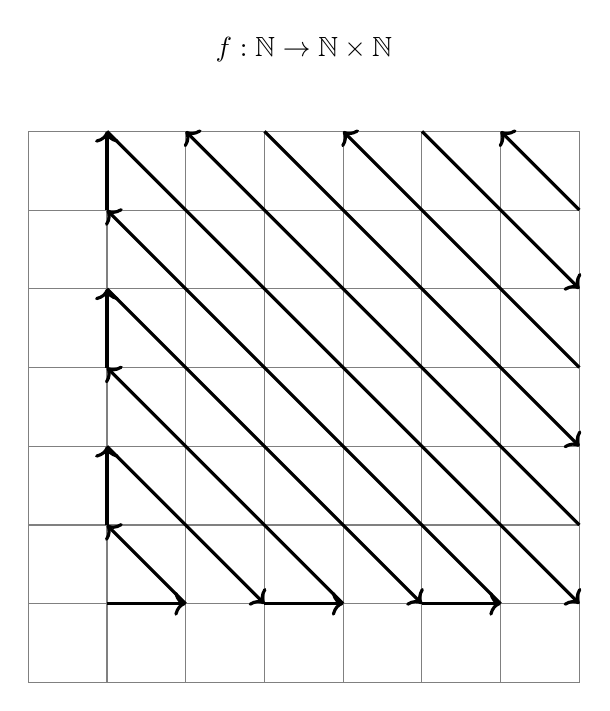
\begin{tikzpicture}[style={line width=0.4mm}]
   \tkzInit[xmax=7,ymax=7,xmin=0,ymin=0]
   \tkzGrid
   \tkzAxeXY
   \draw[->](1,1)  --  (2,1);
   \draw[->](2,1)  --  (1,2);
   \draw[->](1,2)  --  (1,3);
   \draw[->](1,3)  --  (3,1);
   \draw[->](3,1)  --  (4,1);
   \draw[->](4,1)  --  (1,4);
   \draw[->](1,4)  --  (1,5);
   \draw[->](1,5)  --  (5,1);
   \draw[->](5,1)  --  (6,1);
   \draw[->](6,1)  --  (1,6);
   \draw[->](1,6)  --  (1,7);
   \draw[->](1,7)  --  (7,1);
   \draw[->](7,2)  --  (2,7);
   \draw[->](3,7)  --  (7,3);
   \draw[->](7,4)  --  (4,7);
   \draw[->](5,7)  --  (7,5);
   \draw[->](7,6)  --  (6,7);
  \tkzText[above](3.5,7.75){$f:\N \rightarrow \N \times \N$}
\end{tikzpicture}
\end{center}
\newpage
\begin{flushleft}
Just as $f$ describes a 1-1 correspondence between a single natural number and a pair of natural numbers, we can imagine a similar correspondence that maps a natural number to pair of integers expressed as a ratio. Only two quadrants need to mapped, one without negative numbers and one with only one negative number as the other two would be equivalent. Since many ratios of natural numbers would be reducible to the same value, many of the points in the mapping below would be skipped over. For example, the points $(1,2)$ and $(2,4)$ would both be mapped to the rational value $\frac{1}{2}$ and so the second point in the path would be skipped. To avoid division by zero, we avoid mapping to the x-axis. We start our path at (0,1), which corresponds to the rational number 0, which is determined by diving the x-coordinate by the y-coordinate. We follow a similar path as the graph above with the added caveat that the second quadrant is also traversed by following a mirrored path as the first quadrant. When a given rational number is repeated such as (1,2) and (2,4), we skip the subsequent coordinates and continue our indexing from the natural numbers.
\end{flushleft}

\begin{center}
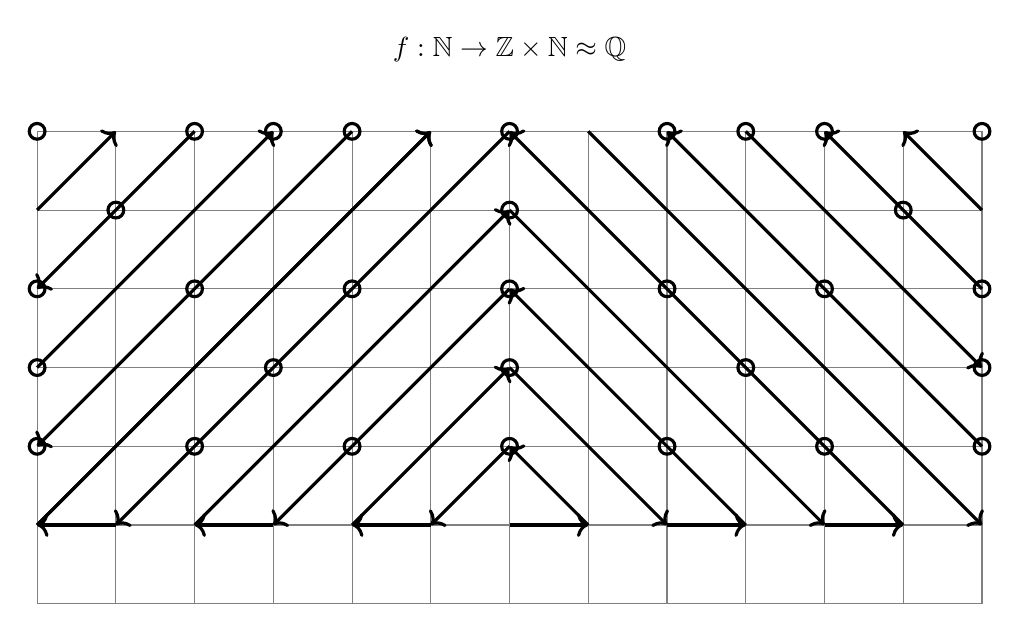
\begin{tikzpicture}[style={radius=.1, line width=0.4mm}]
   \tkzInit[xmax=6,ymax=6,xmin=-6,ymin=0]
   \tkzGrid
   \tkzAxeXY
   \draw[->](0,1)  --  (1,1);
   \draw[->](1,1)  --  (0,2);
   \draw[->](0,2)  --  (-1,1);
   \draw[->](-1,1)  --  (-2,1);
   \draw[->](-2,1)  --  (0,3);
   \draw[->](0,3)  --  (2,1);
   \draw[->](2,1)  --  (3,1);
   \draw[->](3,1)  --  (0,4);
   \draw[->](0,4)  --  (-3,1);
   \draw[->](-3,1)  --  (-4,1);
   \draw[->](-4,1)  --  (0,5);
   \draw[->](0,5)  --  (4,1);
   \draw[->](4,1)  --  (5,1);
   \draw[->](5,1)  --  (0,6);
   \draw[->](0,6)  --  (-5,1);
   \draw[->](-5,1)  --  (-6,1);
   \draw[->](-6,1)  --  (-1,6);
   \draw[->](1,6)  --  (6,1);
   \draw[->](6,2)  --  (2,6);
   \draw[->](-6,1)  --  (-1,6);
   \draw[->](3,6)  --  (6,3);
   \draw[->](6,4)  --  (4,6);
   \draw[->](6,5)  --  (5,6);
   \draw[->](-2,6)  --  (-6,2);
   \draw[->](-6,3)  --  (-3,6);
   \draw[->](-4,6)  --  (-6,4);
   \draw[->](-6,5)  --  (-5,6);
   \draw (0,2) circle;
   \draw (0,3) circle;
   \draw (0,4) circle;
   \draw (0,5) circle;
   \draw (0,6) circle;
   \draw (2,4) circle;
   \draw (3,6) circle;
   \draw (2,6) circle;
   \draw (4,2) circle;
   \draw (4,6) circle;
   \draw (6,2) circle;
   \draw (6,3) circle;
   \draw (6,4) circle;
   \draw (2,2) circle;
   \draw (3,3) circle;
   \draw (4,4) circle;
   \draw (5,5) circle;
   \draw (6,6) circle;
   \draw (-2,4) circle;
   \draw (-3,6) circle;
   \draw (-2,6) circle;
   \draw (-4,2) circle;
   \draw (-4,6) circle;
   \draw (-6,2) circle;
   \draw (-6,3) circle;
   \draw (-6,4) circle;
   \draw (-2,2) circle;
   \draw (-3,3) circle;
   \draw (-4,4) circle;
   \draw (-5,5) circle;
   \draw (-6,6) circle;
  \tkzText[above](0,6.75){$f:\N \rightarrow \Z \times \N \approx \Q$}
\end{tikzpicture}
\end{center}

\end{enumerate}
\end{document}